

\tikzset{every picture/.style={line width=0.75pt}} %set default line width to 0.75pt        

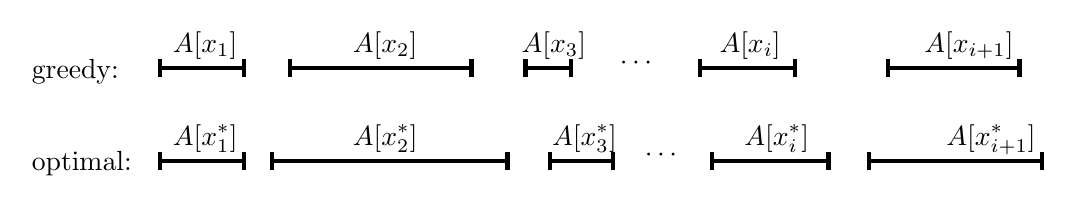
\begin{tikzpicture}[x=0.5pt,y=0.5pt,yscale=-1,xscale=1]
%uncomment if require: \path (0,142); %set diagram left start at 0, and has height of 142

%Straight Lines [id:da9640237890291299] 
\draw [line width=1.5]    (111,47) -- (171.5,47) ;
\draw [shift={(171.5,47)}, rotate = 180] [color={rgb, 255:red, 0; green, 0; blue, 0 }  ][line width=1.5]    (0,6.71) -- (0,-6.71)   ;
\draw [shift={(111,47)}, rotate = 180] [color={rgb, 255:red, 0; green, 0; blue, 0 }  ][line width=1.5]    (0,6.71) -- (0,-6.71)   ;
%Straight Lines [id:da3355888679808179] 
\draw [line width=1.5]    (205,47) -- (336,47) ;
\draw [shift={(336,47)}, rotate = 180] [color={rgb, 255:red, 0; green, 0; blue, 0 }  ][line width=1.5]    (0,6.71) -- (0,-6.71)   ;
\draw [shift={(205,47)}, rotate = 180] [color={rgb, 255:red, 0; green, 0; blue, 0 }  ][line width=1.5]    (0,6.71) -- (0,-6.71)   ;
%Straight Lines [id:da09988799250468405] 
\draw [line width=1.5]    (375,47) -- (408,47) ;
\draw [shift={(408,47)}, rotate = 180] [color={rgb, 255:red, 0; green, 0; blue, 0 }  ][line width=1.5]    (0,6.71) -- (0,-6.71)   ;
\draw [shift={(375,47)}, rotate = 180] [color={rgb, 255:red, 0; green, 0; blue, 0 }  ][line width=1.5]    (0,6.71) -- (0,-6.71)   ;
%Straight Lines [id:da8137923006965678] 
\draw [line width=1.5]    (501,47) -- (569.5,47) ;
\draw [shift={(569.5,47)}, rotate = 180] [color={rgb, 255:red, 0; green, 0; blue, 0 }  ][line width=1.5]    (0,6.71) -- (0,-6.71)   ;
\draw [shift={(501,47)}, rotate = 180] [color={rgb, 255:red, 0; green, 0; blue, 0 }  ][line width=1.5]    (0,6.71) -- (0,-6.71)   ;
%Straight Lines [id:da2017441450503047] 
\draw [line width=1.5]    (637,47) -- (732,47) ;
\draw [shift={(732,47)}, rotate = 180] [color={rgb, 255:red, 0; green, 0; blue, 0 }  ][line width=1.5]    (0,6.71) -- (0,-6.71)   ;
\draw [shift={(637,47)}, rotate = 180] [color={rgb, 255:red, 0; green, 0; blue, 0 }  ][line width=1.5]    (0,6.71) -- (0,-6.71)   ;
%Straight Lines [id:da517279355434781] 
\draw [line width=1.5]    (111,114) -- (171.5,114) ;
\draw [shift={(171.5,114)}, rotate = 180] [color={rgb, 255:red, 0; green, 0; blue, 0 }  ][line width=1.5]    (0,6.71) -- (0,-6.71)   ;
\draw [shift={(111,114)}, rotate = 180] [color={rgb, 255:red, 0; green, 0; blue, 0 }  ][line width=1.5]    (0,6.71) -- (0,-6.71)   ;
%Straight Lines [id:da38986625384521667] 
\draw [line width=1.5]    (192,114) -- (362,114) ;
\draw [shift={(362,114)}, rotate = 180] [color={rgb, 255:red, 0; green, 0; blue, 0 }  ][line width=1.5]    (0,6.71) -- (0,-6.71)   ;
\draw [shift={(192,114)}, rotate = 180] [color={rgb, 255:red, 0; green, 0; blue, 0 }  ][line width=1.5]    (0,6.71) -- (0,-6.71)   ;
%Straight Lines [id:da05974740127099276] 
\draw [line width=1.5]    (393,114) -- (438,114) ;
\draw [shift={(438,114)}, rotate = 180] [color={rgb, 255:red, 0; green, 0; blue, 0 }  ][line width=1.5]    (0,6.71) -- (0,-6.71)   ;
\draw [shift={(393,114)}, rotate = 180] [color={rgb, 255:red, 0; green, 0; blue, 0 }  ][line width=1.5]    (0,6.71) -- (0,-6.71)   ;
%Straight Lines [id:da16736606457108671] 
\draw [line width=1.5]    (510,114) -- (594,114) ;
\draw [shift={(594,114)}, rotate = 180] [color={rgb, 255:red, 0; green, 0; blue, 0 }  ][line width=1.5]    (0,6.71) -- (0,-6.71)   ;
\draw [shift={(510,114)}, rotate = 180] [color={rgb, 255:red, 0; green, 0; blue, 0 }  ][line width=1.5]    (0,6.71) -- (0,-6.71)   ;
%Straight Lines [id:da6988626492100889] 
\draw [line width=1.5]    (623,114) -- (748,114) ;
\draw [shift={(748,114)}, rotate = 180] [color={rgb, 255:red, 0; green, 0; blue, 0 }  ][line width=1.5]    (0,6.71) -- (0,-6.71)   ;
\draw [shift={(623,114)}, rotate = 180] [color={rgb, 255:red, 0; green, 0; blue, 0 }  ][line width=1.5]    (0,6.71) -- (0,-6.71)   ;

% Text Node
\draw (16,38) node [anchor=north west][inner sep=0.75pt]   [align=left] {greedy:};
% Text Node
\draw (118,18.5) node [anchor=north west][inner sep=0.75pt]   [align=left] {$\displaystyle A[ x_{1}$]};
% Text Node
\draw (248,18.5) node [anchor=north west][inner sep=0.75pt]   [align=left] {$\displaystyle A[ x_{2}$]};
% Text Node
\draw (370,18.5) node [anchor=north west][inner sep=0.75pt]   [align=left] {$\displaystyle A[ x_{3}$]};
% Text Node
\draw (513,18.5) node [anchor=north west][inner sep=0.75pt]   [align=left] {$\displaystyle A[ x_{i}$]};
% Text Node
\draw (661,18.5) node [anchor=north west][inner sep=0.75pt]   [align=left] {$\displaystyle A[ x_{i+1}$]};
% Text Node
\draw (16,105) node [anchor=north west][inner sep=0.75pt]   [align=left] {optimal:};
% Text Node
\draw (118,85.5) node [anchor=north west][inner sep=0.75pt]   [align=left] {$\displaystyle A[ x^{*}_{1}$]};
% Text Node
\draw (248,85.5) node [anchor=north west][inner sep=0.75pt]   [align=left] {$\displaystyle A[ x^{*}_{2}$]};
% Text Node
\draw (392,85.5) node [anchor=north west][inner sep=0.75pt]   [align=left] {$\displaystyle A[ x^{*}_{3}$]};
% Text Node
\draw (531,85.5) node [anchor=north west][inner sep=0.75pt]   [align=left] {$\displaystyle A[ x^{*}_{i}$]};
% Text Node
\draw (677,85.5) node [anchor=north west][inner sep=0.75pt]   [align=left] {$\displaystyle A[ x^{*}_{i+1}$]};
% Text Node
\draw (441,36.5) node [anchor=north west][inner sep=0.75pt]   [align=left] {$\displaystyle \cdots $};
% Text Node
\draw (459,103.5) node [anchor=north west][inner sep=0.75pt]   [align=left] {$\displaystyle \cdots $};


\end{tikzpicture}

